% Map of the West Indies
\begin{figure}[H]
    \centering
	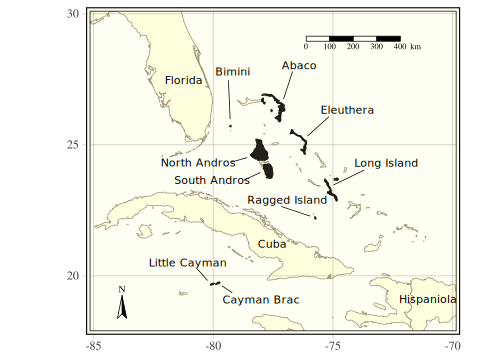
\includegraphics[width=0.8\textwidth]{figures/map.pdf}
	\caption{Map of the West Indies with sampled islands highlighted in black.}
	\label{fig:map}
\end{figure}

% Classification accuracy of SVMs
\begin{figure}[H]
    \centering
	\includegraphics[width=\textwidth]{figures/classif_svm_pca.png}
	\caption{Distributions of classification accuracy across all SVM machines (100 replicates of 5 cross-validation bins each). The dashed line represents the density of a corresponding null binomial distribution, which would be expected under random guessing (testing sets with 20\% of the observations for each island and success probability of $1/3$). Inset plots show the corresponding average confusion matrices and represent the proportion of lizards from each habitat (columns) reassigned in each other habitat (rows), with an interpretation guide in the right panel. P-values indicate deviations of the mean classification accuracy to the expected null binomial distribution. *, P < 0.05}
	\label{fig:classif_svm_pca}
\end{figure}

% Boxplots and analyses of variance
\begin{sidewaysfigure}
    \centering
	\includegraphics[width=18cm]{figures/figure_anova.png}
	\caption{Dewlap coloration varies between habitat-types along different dimensions on different islands. (A) Boxplots show the distribution of the data for the five islands with significant differences in dewlap coloration between habitat (P-values in Fig. \ref{fig:classif_svm_pca}), along the first four principal components. We report the P-values of univariate analyses of variance conducted for each island (see Methods). Horizontal bars indicate \textit{post hoc} significant contrasts at a 0.05 error rate (see Methods). *, P < 0.05. (B) Mapping of the reflectance at various wavelengths onto the principal components. Note that PC1 largely represents brightness.}
	\label{fig:boxplots}
\end{sidewaysfigure}